\documentclass[a4paper,colorinlistoftodos, 10pt]{article}
\input{../../article_preamble.tex}

\title{Mandatory Assignment 1 - Life Insurance Mathematics}
\author{Ditte Gottlieb}
\date{\today}

\begin{document}
\maketitle

\section*{Stat230 27. mai 2014: Oppgave 1}

Per Pettersen changes employer at his 46th birthday. He is given 200000 kroner from
the company’s pension plan. He invest this money in a fund that guarantees 8 \% annual
interest rate, and leaves it there until his retirement at age 60. He plans 25 annual
withdrawals (x) from this fund, the first on his 61st birthday. Our task is to find x.\newline

\noindent The timeline is illustrated in the following figure.
\begin{figure}[ht]
\centering
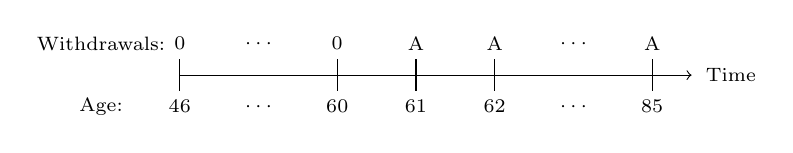
\begin{tikzpicture}
\draw[->] (4,0) -- (10.5,0);
\draw (4,-0.2) -- (4,0.2);
\draw (6,-0.2) -- (6,0.2);
\draw (7,-0.2) -- (7,0.2);
\draw (8,-0.2) -- (8,0.2);
\draw (10,-0.2) -- (10,0.2);
\draw (4, -0.4) node{{\scriptsize 46}};
\draw (5, -0.4) node{{\scriptsize $\cdots$}};
\draw (6, -0.4) node{{\scriptsize 60}};
\draw (7, -0.4) node{{\scriptsize 61}};
\draw (8, -0.4) node{{\scriptsize 62}};
\draw (9, -0.4) node{{\scriptsize $\cdots$}};
\draw (10, -0.4) node{{\scriptsize 85}};
\draw (4, 0.4) node{{\scriptsize 0}};
\draw (5, 0.4) node{{\scriptsize $\cdots$}};
\draw (6, 0.4) node{{\scriptsize 0}};
\draw (7, 0.4) node{{\scriptsize A}};
\draw (8, 0.4) node{{\scriptsize A}};
\draw (9, 0.4) node{{\scriptsize $\cdots$}};
\draw (10, 0.4) node{{\scriptsize A}};
\draw (3, 0.4) node{{\scriptsize Withdrawals:}};
\draw (3, -0.4) node{{\scriptsize Age:}};
\draw (11, 0) node{{\scriptsize Time}};
\end{tikzpicture}
\caption{Illustration of the pension withdrawals.}
\end{figure}


\noindent I have also changed this!
\begin{equation*}
    H = 200000 (1 + 0.08)^{15} = 634433.8.
\end{equation*}
He wishes to make annual withdrawals of the same amount meaning that $A = A_1 = \cdots = A_{25}$. We can thus use that we know that $H$ has to be equal to the sum of the discounted withdrawals i.e.
\begin{equation*}
    H = A\sum_{j=1}^{25} v^j.
\end{equation*}
From this is follows that 
\begin{equation*}
    A = \frac{H}{\sum_{j=1}^{25} v^j} = 59433.
\end{equation*}
Thus he will make an annual withdrawal of 59433 kr. from the fond.



\section*{Stat230 1. juni 2006: Oppgave 2}

A bond is a contract obligating one party, the borrower, or bond issuer, to pay the other party, the lender or bondholder, a series of future payments defined by the face value, $F$, and the coupon rate, $c$. At the end of each future period the borrower pays $cF$ to the lender. The bond matures after $N$ periods with a final coupon payment and a simultaneous payment of the redemption value $C$. Usually $C$ is equal to $F$. Investors (lenders) require a yield to maturity of $i\geq 0$ effective per period. The price, $P$, is the present value of future cash flows paid to the bondholder. We are asked to show that these five values are related by the following equation.
\begin{equation*}
    P = cF\frac{1-v^N}{i} + Cv^N
\end{equation*}
where $v = 1/(1+i)$. The process is illustrated by the following timeline.

\begin{figure}[ht]
\centering
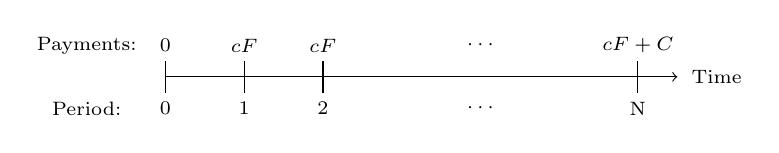
\begin{tikzpicture}
\draw[->] (4,0) -- (10.5,0);
\draw (4,-0.2) -- (4,0.2);
\draw (5,-0.2) -- (5,0.2);
\draw (6,-0.2) -- (6,0.2);
\draw (10,-0.2) -- (10,0.2);
\draw (4, -0.4) node{{\scriptsize 0}};
\draw (5, -0.4) node{{\scriptsize 1}};
\draw (6, -0.4) node{{\scriptsize 2}};
\draw (8, -0.4) node{{\scriptsize $\cdots$}};
\draw (10, -0.4) node{{\scriptsize N}};
\draw (4, 0.4) node{{\scriptsize 0}};
\draw (5, 0.4) node{{\scriptsize $cF$}};
\draw (6, 0.4) node{{\scriptsize $cF$}};
\draw (8, 0.4) node{{\scriptsize $\cdots$}};
\draw (10, 0.4) node{{\scriptsize $cF + C$}};
\draw (3, 0.4) node{{\scriptsize Payments:}};
\draw (3, -0.4) node{{\scriptsize Period:}};
\draw (11, 0) node{{\scriptsize Time}};
\end{tikzpicture}
\caption{Illustration of the payment stream.}
\end{figure}

\noindent We are asked to find the present value $P$ of all future payments. As illustrated in the figure above, we pay $cF$ in each timestep $t=1,\dots,N$ while in the final timestep we also pay the redemption value $C$. Using that the present value is the sum of the discounted payments, we find 
\begin{align*}
P = cF(v + \cdots + v^N) + Cv^N.
\end{align*}
So we wish to show that 
\begin{equation*}
cF(v + \cdots + v^N) = cF\frac{1-v^N}{i}.
\end{equation*}
For this, we use the formula for a finite geometric series such that
\begin{align*}
cF(v + \cdots + v^N) & = cF\Big(\sum_{k=0}^N (v^k) - 1\Big) \\
& = cF\Big(\frac{1-n^{N+1}}{1-v} - 1\Big) \\
& = cF\frac{1-v^{N+1} - (1-v)}{iv} \\
& = cF\frac{v(1-v^N)}{iv} \\
& = cF\frac{1-v^N}{i}
\end{align*}
where we have also used that $1-v = iv$.


\section*{M262 9. juni 2000: Oppgave 2}
Consider a loan of value $H$ with duration $N$ years, and assume that all payments fall at the turn of the year. The interests are payed \emph{in advance}. Let $i$ describe the interest rate in arrears. We use the following notation:
\begin{itemize}
\item $F_t = \text{payment at end of year } t$
\item $R_t = \text{remaining dept right after $F_t$ has been paid}$
\item $A_t = \text{the amortization amount paid at the end of year } t$
\end{itemize}
We are asked to solve the following:
\begin{enumerate}
\item Explain the interpretation of $v=1/(1+i)$ and $d = iv$.

The factor $v=1/(1+i)$ is the discounting factor. We can apply this for finding the present value for a payment which is planed some time into the future. 

The factor $d = iv$ is the discounted interest rate. In this setup, we pay the interests in advance, but since $i$ is the interest rate in arrears, we need this discounted interest rate.

\item Explain that with $F_0=R_N=0$, we have that
\begin{align}
A_t & = F_t + dR_t, \quad t = 0,1, \dots, N. \label{first} \\
A_t & = R_{t-1} - vR_t, \quad t = 1, \dots, N. \label{second}
\end{align}
At time $t=0$, when the loan is taken, we will pay interest of the entire loan value. This corresponds to $A_0 = dR_0 = dH$. The following $N-1$ years, we will pay some installment as well as interest of the remaining dept. This corresponds to $A_i = F_i + dR_i$ for $i=1,\dots, N-1$. Finally, in the last year $N$, we pay the final installment but no interest, since no dept is left after $F_N$ has been paid. Thus $A_N=F_N$ and from this (\ref{first}) follows.

Since $R_t$ describes the remaining dept right after $F_t$ is paid, we can describe the amortization amout $A_t$ paid at the end of year $t$, as the difference in the remaining dept after $F_{t-1}$ has been paid (i.e $R_{t-1}$) and after $F_t$ has been paid (i.e. $R_t$). However we then of course have to discount the value of $R_t$ such that the value of each of the remaining depts are evaluated at the same point in time. Thus follows \ref{second}.


\item Show that 
\begin{equation*}
R_n = \sum_{t=1}^{N-n} A_{t+n} v^{t-1} \quad \text{and}\quad H = \sum_{t=0}^N A_t v^t.
\end{equation*}

From above, we have that $A_t=R_{t-1} - vR_t$. Using this in a recursive matter, we find that
\begin{align*}
R_n & = A_{n+t} + vR_{n+1} \\
& = A_{n+t} + v(A_{n+2} + vR_{n+2}) \\
& = A_{n+t} + vA_{n+2} + v^2(A_{n+3} + vR_{n+3}) \\
& \; \vdots \\
& = A_{n+t} + vA_{n+2} + v^2A_{n+3} + \cdots + v^{N-n-1}A_{n+N-n} \\
& = \sum_{t=1}^{N-n} A_{n+t}v^{t-1}.
\end{align*}
To show the second result, we use that the loan value $H$ is equal to the sum of the installments such that 
\begin{align*}
H & = \sum_{t=0}^N F_t \\
& = \sum_{t=0}^N (A_t - dR_t) \\
& = A_0 - dR_0 + \sum_{t=1}^N (R_{t-1} - vR_t - dR_t) \\
& = A_0 - dR_0 + \sum_{t=1}^N (R_{t-1} - (v + d)R_t) \\
& = A_0 - dR_0 + \sum_{t=1}^N \Big(
    \sum_{k=1}^{N-(t-1)} A_{k+(t-1)} v^{k-1} - 
    \sum_{k=1}^{N-t} A_{k+t} v^{k-1}
    \Big) \\
& = A_0 - dR_0 + \sum_{t=1}^N A_t v^{t-1} \\
& = A_0 - d\sum_{t=1}^N A_t v^{t-1} + \sum_{t=1}^N A_t v^{t-1} \\
& = A_0 + (1-d)\sum_{t=1}^N A_t v^{t-1} \\
& = A_0 + \sum_{t=1}^N A_t v^t \\
& = \sum_{t=0}^N A_t v^t.
\end{align*}
Here we have used that 
\begin{equation*}
v + d = v + iv = v(1+i) = 1\quad\text{and}\quad 1-d = 1-iv = \frac{1+i-i}{1+t} = v
\end{equation*}
and in the fifth line, we have used that all but one of the elements of the sums cancel out with eachother.

\item What is the amortization amount for an annuity loan with advance interest and for a serial loan with advance interest?

In an annuity loan with advance interest, we have that $A_t = A$ for $t=1,\dots,N$ and $A_0 = dR_0 = dH$. So since we from above have that 
\begin{equation*}
H = \sum_{t=0}^N A_tv^t = A_0 + A\sum_{t=1}^N v^t,
\end{equation*}
we have that the amortization amount for an annuity loan with advance interest becomes
\begin{equation*}
A = \frac{H - A_0}{\sum_{t=1}^N v^t}.
\end{equation*}

For a serial loan with advance interest, we instead have that $F_t = \frac{H}{N}$ for $t=1,\dots, N$ while $F_0=0$. Furthermore, we have that the interest at $t=0$ is $dR_0=dH$ while for $t=1,\dots,N$, the remaining dept becomes $d(H-t\frac{H}{N})$. From this is follows that the amortization amount for a serial loan with advance interest becomes
\begin{align*}
A_t & = F_t + dR_t \\
& = \frac{H}{N} + dH\Big(1-\frac{t}{N}\Big) \\
& = \frac{H}{N} + dH\frac{N-t}{N} \\
& = H\Big(\frac{1}{N} + d\frac{N-t}{N}\Big).
\end{align*}
for $t=1,\dots,N$.

\item Let $K$ be the market value of the loan. The effective interest for the lender is defined by the equation 
\begin{equation}
    K = \sum_{t = 0}^N A_tv_e^t.
\end{equation}
Show that 
\begin{equation}\label{K-to-find}
    K = H\frac{d}{d_e} + (1-\frac{d}{d_e})\sum_{t=1}^N F_t v_e^t.
\end{equation}

Note: This exercise is not completed. Using the different quantities derived above, we find that 
\begin{align*}
K & = \sum_{t = 0}^N A_tv_e^t \\
& = \sum_{t = 0}^N (F_t + dR_t)v_e^t \\
& = \sum_{t = 1}^N F_tv_e^t + d \sum_{t = 0}^N \frac{A_t - F_t}{d_e}v_e^t \\
& = (1-\frac{d}{d_e}) \sum_{t = 1}^N F_tv_e^t + \frac{d}{d_e}\sum_{t=0}^N A_tv_e^t.
\end{align*}
Thus we have found the final term of (\ref{K-to-find}). Thus let us consider the last term above
\begin{align*}
\frac{d}{d_e}\sum_{t=0}^N A_tv_e^t & = \frac{1-v}{d_e}A_0 + \frac{d}{d_e}\sum_{t=1}^N A_tv_e^t \\
& = \frac{d}{d_e}H - \frac{v}{d_e} A_0 + \frac{d}{d_e}\sum_{t=1}^N A_tv_e^t
\end{align*}
where we have used that $d=1-v$ and $A_0=dH$. Now it remains to show that 
\begin{equation*}
\frac{d}{d_e}\sum_{t=1}^N A_tv_e^t - \frac{v}{d_e} A_0 = 0.
\end{equation*}
\end{enumerate}
\end{document}
